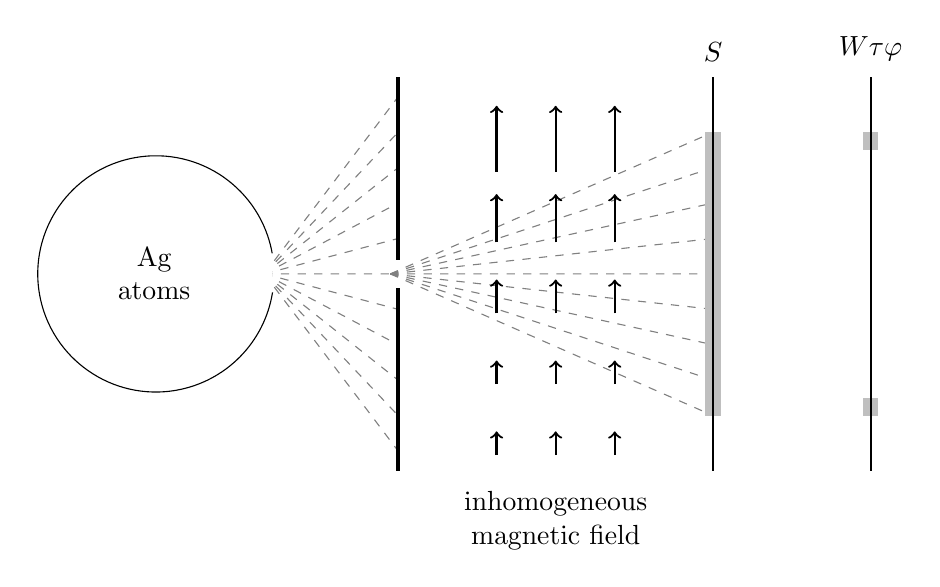
\begin{tikzpicture}[every text node part/.style={align=center}]
    \foreach \i in {0,1,...,10} {
    \draw[dashed,gray] (0.8,0) -- (2.5,2.25-0.45*\i);
    };
    \draw[fill=white] (0.9,1.5*sin 10) arc (10:351:1.5);

    \draw[ultra thick] (2.5,2.5)--(2.5,0.18);
    \draw[ultra thick] (2.5,-0.18)--(2.5,-2.5);
    \draw (-0.6,0)  node {Ag\\ atoms};

    \foreach \i in {1,...,9} {
    \draw[dashed,gray] (2.4,0) -- (6.5,2.25-0.45*\i);
    };

    \foreach \i in {0,1,...,4} {
      \foreach \j in {1,2,3} {
    \draw[thick,->] (3+0.75*\j,-2.3+0.9*\i) -- (3+0.75*\j,-2+0.9*\i^1.1);
    };};

    \fill[lightgray] (6.5-0.1,2.25-0.45*9) rectangle (6.5+0.1,2.25-0.45);
    \draw[thick] (6.5,-2.5)--(6.5,2.5) node[above=2pt] {$S$};

    \fill[lightgray] (8.5-0.1,2.25-0.45*9) rectangle (8.5+0.1,2.25-8.5*0.45);
    \fill[lightgray] (8.5-0.1,2.25-0.45*1.5) rectangle (8.5+0.1,2.25-0.45);
    \draw[thick] (8.5,-2.5)--(8.5,2.5) node[above=2pt] {$W\tau\varphi$};
    \draw (4.5,-2.5) node[below=4pt] {inhomogeneous \\ magnetic field};
\end{tikzpicture}
